\documentclass[12pt,fleqn]{article}\usepackage{../../common}
\begin{document}
Ders 1.27

Bu derse vereceğim ödevi tarif ederek başlayayım, ödevde Poisson denkleminin
çözümü, ama sınırları kare değil çember olan bir ızgarada çözmenizi
isteyeceğim. Çözülecek denklem

$$
-u_{xx} - u_{yy} = 4
$$

Eşitliğin sağ tarafında sabit olduğu için $f$ çarpı $v$ sonrası alınacak
entegraller daha basit oluyor tabii, sabit çarpı deneme fonksiyonu, kolay hesap.
Sınırda, çember üzerinde, $u = 0$ şartını koyuyoruz. Bu sistemi çözeceğiz.

Analitik çözümün ne olduğunu görmek zore değil, $u = 1 - x^2 - y^2$ çözüm.
Yerine koyarsak doğrulaması kolay, iki kere $x$ türevi 2, $y$ türevi 2, toplam
4.

Çember içindeki ızgaraya önce bir poligonla başlıyorum. Bu arada araştırma
sorusu bağlamında aklımdaki sorulardan biri ızgara şekline göre hesabın ortaya
çıkaracağı hata miktarı. Bazı ızgaralar diğerlerinden daha iyi olabilir.

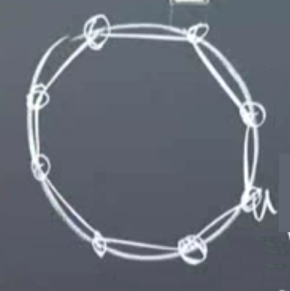
\includegraphics[width=10em]{compscieng_1_27_01.png}

Sınır şartımızı hatırlarsak düz cizgilerin çembere değdiği noktalarda $u = 0$.

$M$ tane köşe olsun, ve orta noktadan köşelere çizgiler çekerek üçgenler
oluşturalım, altta üçgenlerden biri görülüyor,

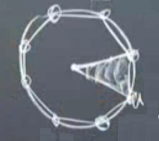
\includegraphics[width=10em]{compscieng_1_27_02.png}

Üçgenin alt iki köşesinde tabii ki $u = 0$ şartı geçerli. İki üçgen arasındaki
sınırda ise doğal sınır şartı denilen Neumann şartı geçerli olacak, eğimin
sıfır olma şartı, yani $\ud u / \ud n = 0$. Orijinde ne yapmam gerektiğinden
emin değilim şu anda. 

Gerçek bir problem işte burada. Muhakkak problem biraz yapay, çünkü analitik
çözümün ne olduğunu biliyoruz, ama mesela bu problemde hesap yapmak, hatanın
ne olacağını düşünmek, bunlar ciddi işler. 

Bu problemi çözerken parçasal lineer öğeler (piecewise linear elements)
kullanmanızı isteyeceğim, daha önce bahsettiğim piramitler bunlar. Ama
bazılarınız karesel (quadratic) öğeler kullanmak isterse buna hayır demem.
Bu öğeler daha hassas / doğru sonuçlar verecektir. 

Simdi izgarayi daha detayli sekilde yaratalim. Bir liste yaratacagiz, bu
listede izgara noktalari olacak, bu liste cozum algoritmasina verilecek
ve algoritma oradan devam edecek.

Çember içinde daha önce yarattığımız üçgenlerden iki tanesini yanyana düşünelim,
en sağ üstteki nokta nerededir? $(\cos \pi/8, \sin \pi/8)$ değil mi? Sonra en
soldan en sağa $N$ tane (resimde $N=4$) düğüm daha koyarız, her aralık yatay
eksende $h$ büyüklüğünde olabilir, ve $N h = \cos\pi/8$ tabii ki.

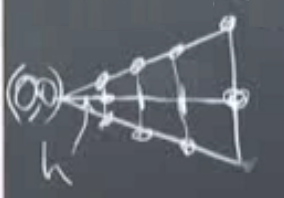
\includegraphics[width=20em]{compscieng_1_27_03.png}












[devam edecek]

Kaynaklar

[1] {\em 18.085 SUMMER 2012 Site},
    \url{https://math.mit.edu/classes/18.085/2012summer.html}

\end{document}
